\documentclass[12pt]{book}

\usepackage{amsfonts,amsmath,amssymb,gensymb,color,soul,graphicx,titlesec,tabu,longtable,array,natbib}
\usepackage[colorlinks,linkcolor=blue,citecolor=blue,urlcolor=blue,pdftitle={Balrog},pdfauthor={Suchyta}]{hyperref}
\usepackage[margin=1in]{geometry}
\usepackage[singlelinecheck=false]{caption}
\usepackage{title,optstable,config,outtable,todonotes}
\bibliographystyle{mn2e_adsurl}


\renewcommand*\chapterautorefname{Chapter}
\renewcommand*\sectionautorefname{Section}
\renewcommand*\subsectionautorefname{Sectiggon}
\renewcommand*\subsubsectionautorefname{Section}

\newcommand{\py}{Python}
\newcommand{\galsim}{GalSim}
\newcommand{\balrog}{\textsc{Balrog}}
\newcommand{\sex}{\textsc{SExtractor}}
\newcommand{\psfex}{\textsc{PSFEx}}
\newcommand{\opt}[1]{\texttt{--#1}}
\newcommand{\inline}{\\[0.4cm]}
\newcommand{\bcmd}[1]{\texttt{\% runbalrog #1}}
\newcommand{\sersic}{S\'{e}rsic}

\newcommand\note[3]{\todo[color=#1, inline, size=\small]{#2: #3}}
\newcommand\notesuchyta[1]{\note{red!50}{EDS}{#1}}

\titleformat{\chapter}[hang]
{\normalfont\huge\bfseries}{\thechapter.}{1em}{}
\titlespacing*{\chapter}{0pt}{0pt}{25pt}

\renewcommand\footnoterule{}
%\widowpenalty=10000


\def\aj{AJ}%
          % Astronomical Journal
\def\apj{ApJ}%
          % Astrophysical Journal
\def\apjl{ApJ}%
          % Astrophysical Journal, Letters
\def\apjs{ApJS}%
          % Astrophysical Journal, Supplement
\def\apss{Ap\&SS}%
          % Astrophysics and Space Science
\def\aap{A\&A}%
          % Astronomy and Astrophysics
\def\aapr{A\&A~Rev.}%
          % Astronomy and Astrophysics Reviews
\def\aaps{A\&AS}%
          % Astronomy and Astrophysics, Supplement
\def\jcap{J. Cosmology Astropart. Phys.}%
          % Journal of Cosmology and Astroparticle Physics
\def\jrasc{JRASC}%
          % Journal of the RAS of Canada
\def\mnras{MNRAS}%
          % Monthly Notices of the RAS
\def\memras{MmRAS}%
          % Memoirs of the RAS
\def\pra{Phys.~Rev.~A}%
          % Physical Review A: General Physics
\def\prb{Phys.~Rev.~B}%
          % Physical Review B: Solid State
\def\prc{Phys.~Rev.~C}%
          % Physical Review C
\def\prd{Phys.~Rev.~D}%
          % Physical Review D
\def\pre{Phys.~Rev.~E}%
          % Physical Review E
\def\prl{Phys.~Rev.~Lett.}%
          % Physical Review Letters
\def\pasp{PASP}%
          % Publications of the ASP
\def\pasj{PASJ}%
          % Publications of the ASJ
\def\nat{Nature}%
          % Nature
\def\aplett{Astrophys.~Lett.}%
          % Astrophysics Letters
\def\physrep{Phys.~Rep.}%
          % Physics Reports
\def\procspie{Proc.~SPIE}%
          % Proceedings of the SPIE
\let\astap=\aap
\let\apjlett=\apjl
\let\apjsupp=\apjs
\let\applopt=\ao


\begin{document}

%\setlength{\textfloatsep}{10pt plus 1.0pt minus 2.0pt}
\setlength{\intextsep}{25pt plus 1.0pt minus 2.0pt}
\let\cleardoublepage\clearpage
\balrogtitlepage
\tableofcontents


\chapter{Introduction}
\label{sec:intro}
\setlength{\parskip}{0pt}
\renewcommand\footnoterule{\kern-3pt \hrule width 2in \kern 2.6pt}

\balrog{} is a package of \py{} code, intended for use
with astronomical imaging data. 
Strictly speaking, \balrog{} is a simulation tool.
However, its ambition is derived from the aspiration to better 
characterize and understand real data.
By performing a set of simulations,
\balrog{}'s intent is to allow observers to infer properties of their images
by directly testing on the images themselves.

The core functionality driving \balrog{}'s design is rather straightforward.
Galaxies are simulated, trivially writing their simulated properties to a \emph{truth catalog}.
Noisy images of the galaxies are then inserted into real data. 
Source detection software runs over the image,
whose measurements for the simulated galaxies
can be directly compared to the truth catalog.
Accordingly, one is able to answer questions about how measured
properties of the image are related to the true properties.

Instead of reinventing the wheel, the \balrog{} pipeline wraps around existing codes,
well known within the Astronomy community.
All galaxy simulations are implemented via
\galsim{}\footnote{\url{https://github.com/GalSim-developers/GalSim}} (Rowe et al., \emph{in prep.})
and source extraction and measurement occurs using
\sex\footnote{\url{https://www.astromatic.net/software/sextractor}} \citep{sextractor}.
\balrog{} facilitates the ease of running these codes en masse over
many images, filling in many of the bookkeeping steps in an automated fashion.

Since different users will have different needs, \balrog{} strives to be as flexible as possible. 
It includes a well defined framework capable 
of implementing a wide variety of simulation possibilites.
The framework allows users to define their own arguments
and functions to plug into \balrog{} when generating simulated galaxies.

In order to maximize convenience,
\balrog{} has been written making our best attempts at user-friendliness.
Example files are packaged with the code so that following installation,
the pipeline is able to run out of the box without specifying any arguments.
Users are encouraged to use and inspect the default example runs 
to become more familiar with the \balrog{} environment.
To preserve an intuitive feel, \balrog{}'s simulation framework mimics ordinary \py{} syntax. 
Where necessary, files and directories are given understandable names.
Numerous errors and warning are handled, printing useful messages
about why the exception was raised.
Log files are automatically written, useful for follow-up degugging
in the cases where exceptions do occur. User configurations are copied into
the output directory, owing to the consideration that every run should be
reproducible from the output.

In this brief introduction, we have merely scratched the surface explaining \balrog{}'s
uses and capabilites. The remainder of the documentation elaborates further.
\autoref{sec:algorithm} enumerates the components of the \balrog{} pipeline, illustrating its algorithm.
Until now, we have been rather vague about practical applications for \balrog{}.
\autoref{sec:motivation} addresses just that, offering some examples of what can be done with \balrog{} outputs.
\autoref{sec:install} discusses what is necessary for installation.
Beyond, the remainder of the document concerns how to configure and run \balrog{}.
\autoref{sec:quick} presents an approach to hit the ground running and quickly get
started with some key features of \balrog{}.
\autoref{sec:quick} is followed by a number of more comprehensive sections,
which spell out all the usage details.
\autoref{sec:cmdline} covers command line arguments, and
\autoref{sec:simrules} establishes how to simulate galaxies within the \balrog{} framework.
The format of \balrog{}'s outputs are explained in \autoref{sec:out}.
\autoref{sec:debug} offers some debugging hints.


\chapter{The \balrog{} Pipeline}
\label{sec:algorithm}

\autoref{sec:intro} briefly introduced the workflow through the \balrog{} pipeline.
The purpose of this section is to characterize the algorithm in full.
The focus here is methodology, not usage instructions. 
The text is organized as follows.
To begin, the workflow of the pipeline as a whole is described in \autoref{sec:workflow}.
This is then subdivided into three sections to be expanded further,
with links to the extended sections inside \autoref{sec:workflow}.
In \autoref{sec:data}, \balrog{}'s required input data is discussed.
In \autoref{sec:galsim}, properties of the simulated galaxies are described,
with a brief conceptual overview of how the properties can be generated
and comments regarding the steps implemented in \galsim{}.
Finally, \balrog{}'s image source detection and measurement is considered in \autoref{sec:processing}.


\section{Workflow}
\label{sec:workflow}

To open this section, we preseent \autoref{fig:flowchart} as a complement to the text,
and as a guide for what is to come.
The figure is a flowchart visually representing \balrog{}.
Roughly speaking, the text steps throgh this flowchart from left to right.
However, as the lines in \autoref{fig:flowchart} indicate, \balrog{} runs trace out more than a single horizontal line through the diagram.
In order to maintain visually clarity and simplicity, \autoref{fig:flowchart} does not include every possible detail of the pipeline.
Rather, it lays out the structure of how the various steps depend on each other.
Effectively, there are two requirements: a set of simulation configurations and some imaging data.
The pipeline's central components are \galsim{} and \sex{}, which operate on these requirements
to produce output catalogs for further analysis.
The following paragraphs comment further.


\begin{figure}[h]
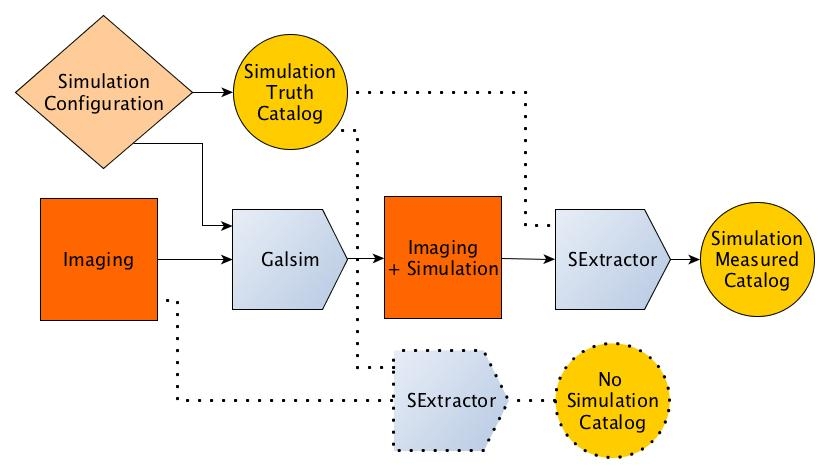
\includegraphics[width=0.9\linewidth]{flowchart.jpg}
\caption{Visualization of \balrog{}'s data flow. Optional (but also default) configurations are represented as dotted connections.}
\label{fig:flowchart}
\end{figure}

The \balrog{}  pipeline begins by opening a log file and parsing the command line options.
The code enforces a number of rules on the user's configurations.
If any errors or warnings occur they are directed to the log file. 
Errors are raised when users make a syntax error and \balrog{} cannot continue.
Generally, warnings occur when something is missing, but the code is able to continue using an internal default. 
Warnings likely, but not always indicate something is not quite right.
The log file remains open, recording messages through the full pipeline.

Next \balrog{} interprets how the user wants to generate their simulated galaxies.
\autoref{sec:galsim} fully prescribes the attributes of these galaxies.
To summarize, each galaxy is composed of one or more \sersic{} profiles.
The user's directives are executed, and  a truth catalog of the galaxy parameters is written.

The code reads in the imaging data into which the simulated galaxies will be drawn.
Refer to \autoref{sec:data} to define what is required of the imaging data in this context.
By default, \sex{} is run over the input image. Please note, at this point no simulated
galaxies have been inserted. However, this command is potentially useful
for reasons discussed further in \autoref{sec:processing}.
An image of each galaxy, commonly known as a postage stamp, is generated and then added atop the input image.
Galaxy postage stamp drawing is treated in \autoref{sec:galsim}.
Once galaxies have been added to the image, \sex{} is called again.
Details of \sex{}'s implementation are deferred to \autoref{sec:processing}.
\sex{} outputs a catalog of the object measurements, which is now ready
for the user to compare with the trutch catalog.


\section{Input Data}
\label{sec:data}

\balrog{} reads in an astronomical image of pixellated flux values.
The data should include a photometric calibration defining
what one ADU count means physically. 
Galaxy simulations are done in apparent magnitude space,
and \balrog{} needs a zeropoint, $m_z$, to convert this to an image ADU level.
$m_z$ is defined in the usual way, where the objects flux, $\mathcal{F}$,
and apparent magnitude, $m$, are related by:
$m - m_ z = -2.5 \log_{10}(\mathcal{F})$.
A default zeropoint of 30 is assumed if one is not otherwise specified.
Required with each image is the image's weight map and PSF model. 
The weight map will be needed when extracting the sources from the image.
At a minimum, the PSF model is necessary for convolving the simulated galaxies
prior to  embedding them in the given image.
It is also obligatory if attempting to fit models to deconvolved measurements of galaxy profiles
during the source measurement process.
The only file type \balrog{} supports for input PSF models is that generated by 
\psfex{}\footnote{\url{www.astromatic.net/software/psfex}} \citep{psfex}.
Readers should be aware that \balrog{} itself does not run \psfex{}.
Thus, generating \psfex{} models constitues a prerequisite users must complete prior to running \balrog{}.
\balrog{} simulations incorporate \galsim{}'s WCS features, and hence
the software requires each image contain sa WCS solution. \balrog{} reads this solution from the image's header.
If no WCS exists in the header, the pipeline enforces a fiducial WCS with a constant pixel scale of 
0.263~arcsec/pixel.\footnote{0.263~arcsec/pixel is the fiducial pixel scale fore DECam.}ß
\balrog{} supports subsampling the input images if desired, meaning galaxies will only be
inserted into a portion of the image.
Once galaxies are simulated, the input image's flux values change by adding the galaxies on top of the original images. 
Algorithmically, this is the only change applied to the input by the entire \balrog{} pipeline.
The weight map and PSF remain unchanged.
Conceptually, the bulk of the undertaking goes into simulationg the galaxies.

\notesuchyta{Is it worth adding some kind of support to generate the \psfex{} model? This introduces some issues doing so, but it might be worthwhile.}

\section{Simulated Galaxies}
\label{sec:galsim}

To simulate galaxies, \balrog{} makes use of \galsim{}. 
It calls \galsim{}'s class for implementing \sersic{} objects to model the galaxies' light distriubtions as \sersic{} profiles. 
By effectively adding together these \sersic{} objects, \balrog{} allows galaxies to be composed of as many superimposed
\sersic{} components as desired. Each of these components has its own \sersic{} index, half light radius, flux,
minor to major axis ratio, and orientation angle. The half light radius is measured along
the major axis, and the orienation angle is measured as the major axis' counter-clockwise rotation
away from the $x$-direction. 
Flux values are generated as magnitudes, then converted to ADU levels 
using the image's zeropoint.
In addtion to its \sersic{} components, each galaxy
shares five parameters which are identical among each \sersic{} component:
two centroid coordinate positions $(x, y)$, two components of lensing reduced shear $(g_1, g_2)$, and magnfication.
The reduced shear follows the usual lensing notation convention, with positive $g_1$ along the $x$-axis,
negative $g_1$ along the $y$-axis, and positive and negative $g_2$ rotated 45\degree{} from the
respective $g_1$ counterparts. Magnification is the usual $\mu = 1 + \kappa$.
To be explictly clear, the shear and magnification are lensing effects applied to a galaxy,
and the axis ratio and orientation angle are intrinsic to the galaxy, as they would in the abscence of lensing.

\balrog{} presents users with a number of different options for how to generate
the truth properties of their galaxies.
Simple types include a constant to be applied commonly to every galaxy or an array containing an element for each galaxy.
Alternatively, values can be sampled from the columns in a catalog file. 
Multiple columns from the same table are automatically jointly sampled.
Last but certainly not least, users can define their own functions which determine the truth paramters of the simulated galaxies.
This is perhaps \balrog{}'s most powerful feature.
It is this functionality which adds the flexibility for \balrog{} to support
virtually anything users can think of and code up in \py{} themselves.
Conveniently, the functions may operate over the galaxies' truth parameters themselves,
allowing one parmeter to be defined in terms of another.

The simulation process runs in a loop with a number of iterations equal to the number of galaxies to be simulated.
A subloop then iterates over the number of \sersic{} profiles the galaxies are composed of.
For each profile, a \sersic{} object is obstantiated with the \sersic{} index,
half light radius, and flux which were generated. Initially these objects are circularly symmetric
so the shearing method is called to create the galaxy's axis ratio, oriented in the appropriate direction.
All these elliptical objects inside the subloop are added together to create the composite galaxy made
of superimposed profiles. Lensing is then applied to the combined object, implementing both the
lensing reduced shear and magnfication.
The PSF model is sampled at the galaxy's centroid position and convolved with the galaxy profile.
Finally, the object is convolved with a top-hat pixel response function
whose scale is equal to that of the local WCS pixel scale.

The galaxy object is then drawn into a postage stamp image. The pixel
scale of the postage stamp is fixed to have the scale of the local WCS at the galaxy's position.
The size of the postage stamp is computed automatically by \galsim{} by dictating that
only a certain small enough fraction of the galaxy's flux is permitted to be lost outside the postage stamp's boundaries.
Additional arguments are also relevant to the final accuracy of the drawn galaxies, but
they go beyond the scope of this section. See \autoref{sec:simrules} or the
\href{http://galsim-developers.github.io/GalSim/structgalsim\_1\_1\_g\_s\_params.html}{galsim.GSParams documentation}
for details. Noise is added to the galaxy's postage stamp by \galsim{}'s functions  for creating CCD-like noise.
The functionality relies on specifying the gain to set the noise level. 
This gain defaults to unity when nothing else if available.
\balrog{} sets the read noise to zero.
The final step in the simulation process is to add the postage stamp to input image, centering the
postage stamp onto the galaxy's generated $(x, y)$ centroid coordinates.


\section{Source Detection and Measurement}
\label{sec:processing}

\balrog{} calls \sex{} at least once, and by default twice throughtout the pipeline.
While this manual is not intended to be a comprehensive guide to
running \sex{}, a few comments are in order.
For those who have never used \sex{}, we direct you to the
\href{https://www.astromatic.net/pubsvn/software/sextractor/trunk/doc/sextractor.pdf}{official \sex{} user manual} 
or alternatively the so-called
\href{http://astroa.physics.metu.edu.tr/MANUALS/sextractor/Guide2source\_extractor.pdf}{Source Extractor for Dummies}
text. We only make remarks about a few of the most pertinent features to be aware of within \balrog{}.

\sex{} runs are configured via roughly a handful of files. 
In this scope, the two relevant ones are what we will call
the \emph{config file}, often denoted with a \texttt{.sex} extension,
and the \emph{param file}, often denoted with a \texttt{.param} extension.
In \balrog{}'s default files shipped with the software, the \sex{} config
file is suffixed with a \texttt{.config} extension for consistency with our terminology.
The config file is allowed to specify any of the arguments which can
also be given as command line arguments.
These set conditions such as the detection thresholds,
the aperture sizes for photometry, the magnitude zeropoint,
and the background subtraction strategy.
The param file is a list of keywords.
Each keyword is a measurment \sex{} will make for every extracted object.

It is the param file which controls whether or not \sex{} will performmodel fits to the galaxies. 
How do to this is documented practically nowhere, but has been passed down by word of mouth in the Astronomy community. 
We will make a small aside to elaborate more thoroughly.
\sex{} includes up to two possible types of models to fit.
One, denoted by the key \texttt{DISK}, is a model with fixed \sersic{} index of $n=1$,
i.e. an exponential.
The other, denoted by the key \texttt{SPHEROID}, is a model with a free \sersic{} index.
\sex{} can fit either of these independently or both simultaneously.
Each model written into and uncommented from the param file is fit,
meaning if just the \texttt{DISK} key is present a disk only model with $n=1$ is fit;
if just the \texttt{SPHEROID} key is present a bulge only model with free $n$ is fit;
and if both \texttt{DISK} and \texttt{SPHEROID} keys are present both the
disk and bulge are fit simultaneously, which is of course different than fitting them independently.
Each model can fit for the flux, magnitude, axis ratio, and orientation angle of the model.
The spheroid model also fits the sersic index and half light radius.
The disk model fits the scale radius, as opposed to the half light radius.
See the \texttt{bulge+disk.param} file included with \balrog{} for the \sex{} names of all the paramters.
The meanings of the names are human readable.

\notesuchyta{I shold probably say something more like ``scarcely documented'', rather than ``practically nowhere'', but the way it is now better represents my true feelings.}

Returning to \balrog{}, the default behavior is to run \sex{} in \emph{association mode}.
For those unfamilar with the terminology, association mode means
\sex{} will only make possible measurements at a predefined list of coordinates.
Here, the list is given as the simulated galaxies' locations. 
Hence, \sex{} is effectively aware of where in the image the galaxies live.
If it finds an object at one of the this coordinates, it extracts it;
but it does not extract objects anwhere else.
This bypasses the need to extract every single object in the image. 
Namely, it  selects against the objects unrelated to the simulated galaxies that 
existed in the image prior to any simulation,
which have no truth information to compare with anyway.
The attractiveness of running in association mode is the reduction in execution time it offers.
In order to avoid simulated galaxies overlapping each other, simulated galaxies should be inserted
into the image at a significantly lower number density than the number density of the image itself.
This means association mode would remove the majority of all objects.
By default \balrog{} configures \sex{} to make a \sersic{} fit to each simulated galaxy.
Because model fitting is a time expnsive step,
association mode offers a significant payoff when using this configuration.
For a large dataset, running \sex{} many times over many images, model fitting 
each object in every run is likely time infeasible.

In addition to running \sex{} over the image with the simulated galaxies,
by default \balrog{} is configured to run \sex{} over the image prior to inserting the simulated galaxies.
This is to confirm if the association mode functionality of \sex{} is genuinely measuring a simulating galaxy.
For example, \balrog{} may happen to place a galaxy into the image a location where a big, bright object already lives.
If the simulated galaxy is rather faint, \sex{} may just interpret its flux as part of the original object, having no
idea the simulated galaxy is even there. The \sex{} run over the pre-simulation image allows users to check
for such occurences if they would like. By default, this calls a param file which does not include model fitting.
For the case described here, there is no benefit to dedicate the additional time needed for model fitting.


\chapter{What Is \balrog{} Good For?}
\label{sec:motivation}

What is \balrog{} good for?


\chapter{Installation}
\label{sec:install}

Installation is a bitch. Let your system administrator worry about it. 
But if you have to do it, here are some steps that \emph{might} work...


\chapter{Quick Start}
\label{sec:quick}

\balrog{} has been designed with flexibility of use in mind. As a necessary consequence, 
a number of different configuration possiblities exist, each of which must be
adequately explained, which quickly expands the length of the documentation.
We realize parsing the entirity of this manual requires some time.
Hence, the intent of the this section is to offer a short primer for a few of the most import features
\balrog{} users will want to become familiar with.
The comprehensive usage instructions are saved for later sections.
The start up pointers below will refer readers to the relevant comprehensive sections for more details.

The fastest way to get started understanding how to configure and use \balrog{} is to
run it using the example files which come packaged with the software, and then examine the input
and output of the run. 
\balrog{} has been set up such that when the executable \py{}
file is called without any command line arguments, it will run over
the example files, filling in defaults as necessary. 
Thus, this inital call is as simple as:
\inline
\bcmd{}
\inline
Referring to \autoref{tab:def}, \texttt{runbalrog} is equivalent to an alias to the file
\texttt{balrog.py} located within the installation directory, labelled like an environment variable as \texttt{\$INSTALLDIR}. We will use these conventions
throughout the documentation. \autoref{sec:input} briefly addresses
the input which was read in for the \texttt{runbalrog} command and \autoref{sec:output} introduces the output
generated during the run.

\section{Input}
\label{sec:input}

\balrog{}'s input comes in two forms, command line arguments and \py{} statements.
The command line arguments can be printed, along with brief help strings by running:
\inline
\bcmd{\opt{help}}
\inline
Furthermore, a complete description of \balrog{}'s command line arguments can be found in \autoref{sec:cmdline}.
Each comes with a default \balrog{} will assume if the user does not supply one.
In brief, the command line parameters are used to specify input images and their properties, as well as configuration
files to use with \sex{}, and a few other variables every \balrog{} run will need to define. 
The default example's image data, weight map, and PSF live in \texttt{\$INSTALLDIR/default\_example/}.
The \sex{} configuration files live in \texttt{\$INSTALLDIR/astro\_config}. 
Command line argument names and default file names are intended to be transparent.

In order to flexibly define how galaxies will be simulated, \balrog{} accepts defined blocks of \py{} code
within the file specified by command line option \opt{config}.
The example's \opt{config} defaults to \texttt{\$INSTALLDIR/config.py}.
Included within this \balrog{} configuration file is support for implementing custom user-defined functions 
and command line arguments.
The core functions defined in the file have a strictly
structured syntax which will be fully described in \autoref{sec:cmdline} and \autoref{sec:simrules}. The syntax is designed to be as \py esque as possible, so
many users will likely be able to extrapolate directly from the examples without reading lengthy documentation. The file also
includes comment lines as a guide. A slightly more sophisticated configuration file can be found in \texttt{\$INSTALLDIR/config2.py}.
These two examples are designed to demonstrate the range of statements available to \balrog{}'s \py{} configuration files.


\section{Output}
\label{sec:output}

All \balrog{} output is saved in subdirectories under the directory chosen by command line option \opt{outdir}.
This directory has defaulted to \texttt{\$INSTALLDIR/default\_example/output} for the example run.
The complete set of output generated by \balrog{} is detailed in \autoref{sec:out};
most relevant for getting started are the \texttt{balrog\_cat} subdirectory and the \texttt{balrog\_log} subdirectory.
\texttt{balrog\_cat} contains \texttt{example.truthcat.sim.fits}, the truth parameters assigned to simulated galaxies
and \texttt{example.measuredcat.sim.fits}, the simulated galaxies' properties as measured in the image by \sex{}.
\texttt{balrog\_log} saves log files useful for debugging \balrog{} runs, including dumps of how the the command line
arguments were parsed, \sex{}'s command line output, and any \balrog{} specific run errors or warning which occured.
\autoref{sec:debug} offers some debugging hints.


\begin{table}[h]
\caption{Definitions used throughout this manual.}
\label{tab:def}
\begin{tabular}{l l}
\underline{\textbf{Name}} & \underline{\textbf{Meaning}} \\
\texttt{\$INSTALLDIR} & Directory where \balrog{} was installed \\
\texttt{runbalrog} & \texttt{\$INSTALLDIR/balrog.py} \\
\end{tabular}
\end{table}


\chapter{Command Line Options}
\label{sec:cmdline}

\balrog{} runs can be configured via command line options.
Two types of options exist. First are the built-in
ones, native to \balrog{}. In addition, \balrog{}
supports a mechanism for users to define their
own command line options.
To print a list of all \balrog{}'s command line options,
both native and user-defined, along with
brief help strings, run:
\inline
\bcmd{\opt{help}}
\inline
\autoref{sec:builtin} further details each
of the native options and \autoref{sec:user}
explains how to create custom options.

\subsection{Built-in Options}
\label{sec:builtin}

\balrog{} includes a number of built-in optional arguments for each run, defining a
variety of parameters such as the input image,
the number of galaxies to simulate, the flux calibration, etc.
Any options which are not specified assume a default value.
The options are intended to be named intuitvely in order
to faciltate ease of use. 
\autoref{tab:opts} lists each option, with a description of 
what it means, including its default.
Abbreviations for each option also exist,
trading clarity for brevity.


\optstab{}

\subsection{User-defined Options}
\label{sec:user}

Within the \config{} file, user's are able to
define their own command line options. This occurs
within the function \argsfunc{}. Passed
to \argsfunc{}  as an argument is \argsparser{},
an object made by \texttt{python}'s
\texttt{argparse.ArgumentParser()}. Arguments
can be added to parser according to the usual
\texttt{argparse} syntax.
For those unfamilar with \texttt{argparse},
\href{http://docs.python.org/2/howto/argparse.html}{this tutorial}
contains many useful examples. A simple example of
\argsfunc{} is copied below.

\setlength{\tabcolsep}{0pt}
\begin{longtabu*} to \linewidth {l X}
\multicolumn{2}{l}{\texttt{def CustomArgs(parser):}}\\
\hspace{20pt} \texttt{parser.add\_argument(} & \texttt{"-cs", "--catalogsample", help="Catalog used to
sample simulated galaxy parameter distriubtions from", type=str, default=None)}
\end{longtabu*}
\setlength{\tabcolsep}{6pt}
\addtocounter{table}{-1}


User-defined options are parsed within the function \parsefunc{},
also part of \config{}.
Passed as an argument to \parsefunc{} is \parseargs{}, equivalent
to an object returned by \texttt{parser.parse\_args()}. Each one of the user's 
command line options becomes an attribute of \parseargs{}. 
A simple version of \parsefunc{} has been included below.

\setlength{\tabcolsep}{0pt}
\begin{longtabu*} to \linewidth {X}
\texttt{def CustomParseArgs(args):}\\
\hspace{20pt} \texttt{thisdir = os.path.dirname( os.path.realpath(\_\_file\_\_) )} \\
\hspace{20pt} \texttt{if args.catalogsample==None:} \\
\hspace{40pt} \texttt{args.catalogsample = os.path.join(thisdir, 'cosmos.fits')}
\end{longtabu*}
\setlength{\tabcolsep}{6pt}
\addtocounter{table}{-1}

\noindent The ability to define and parse one's own command line arguments is intended to make
\balrog{} flexible to conveniently running a wide variety of different
simulation scenarios. These parameters are available to the user 
when setting up the galaxy simulations. How to define these simulations is described in
\autoref{sec:simrules} below.

\chapter{Defining How to Simulate Galaxies}
\label{sec:simrules}

Defining how galaxies should be simulated is controlled within \config{}
in the function \simfunc{}. Passed into the function are three
arguments: \simargs{}, \simrules{}, and \simsamp{}.
\simargs{} refers to the parsed command line arguments,
both native \balrog{} and user-defined.
\simrules{} is an object whose components are overwritten
in order to specify how simulated galaxies are sampled.
\simsamp{} gives access to simulated galaxy parameters
after they have been sampled. \simrules{} and \simsamp{}
will become clearer to follow.

\balrog{} simulates galaxies as $N$ component \sersic{} profiles, 
where $N$ ranges from 1 to as many as desired. Associated
with each of these components are five attributes: a \sersic{} index,
half light radius, magnitude, axis ratio ($b/a$), and orientation
angle ($\beta$). In addition, each simulated galaxy has five attributes
common among each \sersic{} profile: $x$ and $y$-coordinates,
two components of reduced shear ($g_1$, $g_2$), and magnification.
\simfunc{}'s argument \simrules{} is comprised of attributes
for these different galaxy characteristics. Users overwrite
each of \simrules{}'s attributes to define their simulations.
For example the statement to set each galaxy's magnification
to 1 would read:
\inline
\texttt{magnification = 1}
\inline
\simrules{} has 11 attributes in total, whose names are intended to be simple to understand.
These are printed and desribed in \autoref{tab:attr} below.

\vspace{10pt}
\begin{longtabu} to \linewidth {l l}
\caption{Attributes of the rules defining the simulated galxies.} \label{tab:attr}\\
\underline{\textbf{Attribute}} & \underline{\textbf{Meaning}} \\
\texttt{rules.x} & Galaxy centroid $x$-coordinate [pixels], first pixel = 1\\
\texttt{rules.y} & Galaxy centroid $y$-coordinate [pixels], first pixel = 1\\
\texttt{rules.g1} & Reduced shear, $g_1$ component \\
\texttt{rules.g2} & Reduded shear, $g_2$ component \\
\texttt{rules.magnification} & Magnification, $1 + \kappa$ \\
\texttt{rules.nProfiles} & Number of superimposed \sersic{} profiles \\
\texttt{rules.sersicindex} & \sersic{} index \\
\texttt{rules.halflightradus} & \sersic{} half light radius \\
\texttt{rules.magnitude} & Galaxy brightness in magnitudes \\
\texttt{rules.axisratio} & Minor to major axis ratio, $b/a$ \\
\texttt{rules.beta} & Orientaiton angle of major axis (measured from $x$-axis)
\end{longtabu}

\noindent \texttt{rules.sersicindex}, \texttt{rules.halflightradius}, \texttt{rules.magnitude}, \texttt{rules.axisratio},
and \texttt{rules.beta} must be arrays, whose length is equal to \texttt{rules.nProfiles}. For example, simulating
galaxies with both an expontential and a de Vaucouleurs component would read:
\inline
\texttt{rules.nProfiles} = 2 \\
\texttt{rules.sersicindex = [1,4]}

Simulation rules can assume four types. The first is a constant, meaning each of the 
galaxies in the simulated galaxy sample
will have the same value for the selected parameter. 
Rules can also be assigned as an array, equal in length to the number of simulated galaxies. 
Simulated galaxy $i$ for the chosen parameter then assumes the value in element $i$ of
the array.
Additionally, sampling can be drawn from a catlog. Multiple
parameters selected from the same data table are automatically jointly sampled.
Finally a function can be used. Users write their own \texttt{python} function,
then feed this function and its necessary arguments as the arguments to
\balrog{}'s \texttt{Function} command. The defined function must return an
array equal in length to the number of simulated galaxies. Like the array
sampling type, galaxy $i$ will use element $i$ of the returned array.
Currently only positional arguments are supported within the user-defined
functions, but support for keyword arguments will be added.
\texttt{Function} affords both flexiblity and convenience when deciding
how to sample the simulated galaxies. See \config{} for examples
using \texttt{Function} as well as other sampling types.
One simple example of how to implement each of the four different 
types is shown in \autoref{tab:simtype}.

\vspace{10pt}
\setlength{\tabcolsep}{0pt}
\begin{longtabu} to \linewidth {p{1in} l X}
\caption{Syntax examples for each of the simulation types \balrog{} understands.} \label{tab:simtype} \\
\underline{\textbf{Type}} & \multicolumn{2}{l}{\underline{\textbf{Example}}} \\
Constant & \multicolumn{2}{l}{\texttt{rules.g1 = 0}} \\
Array & \texttt{rules.axisratio = [} & \texttt{np.ones(args.ngal)/np.arange(1,args.ngal+1), sampled.axisratio[0]]} \\
Catalog & \texttt{rules.magnitude = [} & \texttt{Catalog(`cosmos.fits', 0, `IMAG'), Catalog(`cosmos.fits', 0, `IMAG')]} \\
Function & \multicolumn{2}{l}{\texttt{rules.g2 = Function(function=NFW2, args=(sampled.x,sampled.y))}}
\end{longtabu}
\setlength{\tabcolsep}{6pt}

The second and fourth examples in \autoref{tab:simtype} makes use of \simsamp{}, the third argument
passed to \simfunc{}. \simsamp{} is an object allowing users to refer to the properties of
the simulated galaxies after they have been sampled. Referring to the second example above,
the first element of \texttt{rules.axisratio} is an array decreasing incrementally from 1 to 0.
The second elemment of \texttt{rules.axisratio} then says to use whatever the sampled values of
 the first element turn out to be. Here, this equates to setting the second element of \texttt{rules.axisratio}
 to the same array as the first element of \texttt{rules.axisratio}, so the use of \simsamp{} is not 
 really necessary. However, return to the fourth example in \autoref{tab:simtype}. Image \texttt{NFW2}
 as a function which takes two arguments, \texttt{x} and \texttt{y}, which returns the $g_2$ component
 of shear at position ($x$,$y$) from an NFW halo with mass $10^{15} M_{\odot}$ whose center lies at (0,0).
 Now image \texttt{sampled.x} and \texttt{sampled.y} were sampled randomly:
 
 \setlength{\tabcolsep}{0pt}
\begin{longtabu} to \linewidth {X}
\texttt{def Random(minimum, maximum, size):} \\
\hspace{20pt}  \texttt{return np.random.uniform(minimum, maximum, size)}\\
\\
\texttt{rules.x = Random(args.xmin, args.xmax, args.ngal)} \\
\texttt{rules.y = Random(args.ymin, args.ymax, args.ngal)}
\end{longtabu}
\setlength{\tabcolsep}{6pt}
\addtocounter{table}{-1}
 
\noindent \texttt{sampled.x} and \texttt{sampled.y} now represent the values
for $x$ and $y$ after the random sampling has occurred. 
Along these lines, \balrog{} can build-up simulations with fairly little recoding between completely
different types of simulations.
\balrog{} makes sure that all the simulation parameters are sampled
in the proper order and will throw an error if something ambiguous was defined
by the user.


\chapter{Output}
\label{sec:out}
Each \balrog{} run generates a number of output files. 
These are organized into a fixed directory structure.
Users indicate the \opt{outdir} command line option, and
the remainder of the naming scheme occurs automatically,
placing files in subdirectories under \opt{outdir}.
Four subdirectories are written, labelled accoring to what
type of files they contain. \autoref{tab:out}
lists the contents of each of these subdirectories,
giving a brief desription of each file. Depending on how
\balrog{} was configured, not necessarily every file
in \autoref{tab:out} will be present in every run.
The \texttt{*} symbol in \autoref{tab:out} will be replaced with
the base name of the input image file. For example,
if the input image is named \texttt{example.fits},
\texttt{*} will be replaced with \texttt{example}.
If the input file name does not end with the \texttt{.fits}
extension, the file name itself is used as the base name.
This does not include any diretories preceeding the file name.
For example, if the input image was given as
\texttt{/Users/somebody/home/image.f}, the
base name would be \texttt{image}.

\outtab{}

\chapter{Debugging}
\label{sec:debug}

Each galaxy is initally simulated within its own image, commonly known as a postage stamp.
The postage stamp pixel values are then added to the appropriate pixel values in the original input image.
To avoid losing a significant portion of a galaxies outside the postage stamp boundaries,
an appropriate postage stamp size must be chosen. 
Bigger postage stamps exclude less flux.
However, the dimensions should not become too large because
larger postage stamps take longer to simulate.
To designate postage stamp sizes, \balrog{} operates using an adjustable threshold, $I_t$.
The postage stamp will be chosen such that the galaxy's surface brightness profile
must fall below $I_t$ before drawing the postage stamp boundaries.

\balrog{} determines its postage stamp sizes conservatively,
airing on the side of making size estimages larger than perhaps strictly required.
To begin, let us assume the simulated galaxies are composed of a single \sersic{} profile.
We will generalize to multiple superimposed profiles to follow.
First a \galsim{} \texttt{Sersic} object is obstantiated.
Such objects within \galsim{} are all initally circularly symmetric. 
The galaxy is then stretched according to its minor to major axis ratio, $\beta$.
$\beta$'s major axis direction is taken to be along the $x$-axis.
Next, the galaxy's lensing shear is applied, expressing the magnitude of its reduced shear 
\mbox{$g = \sqrt{ g_1^2 + g_2^2}$}
as an axis ratio
\mbox{$q = (1-g)/(1+g)$}.
$q$'s major axis is also taken to be along the $x$-direction.
Finishing the lensing effects, the galaxy is magnified, changing its area and flux.
Effectively, the galaxy now exists as an elliptical \sersic{} profile.
Further refferences to the half light radius will refer to that along the major axis.
Please note, the intrinsic axis ratio and lensing shear are applied in the same direction. 
Although the galaxy's simulation specifications need not orient the two identically,
by adopting the same direction, this step has made the galaxy as stretched as possible.
Thus the $x$-direction is necessarily the direction of greatest distance for the galaxy's profile to fall below $I_t$,
and in the abscence of PSF distortions, a large enough postage stamp size along the $x$-axis is certainly 
sufficient in any other direction. Given a \sersic{} surface brightness profile, the distance $r_s$ at which the profile
falls to $I_t$ is easily computed:
\begin{align}
I_t &= I_e \exp \left( -b_n \left[\left( r_s/r_e  \right)^{1/n} -1 \right] \right) \label{eq:sersic} \\
\implies r_s &= r_e \left[1 - \frac{1}{b_n}  \ln \left(\frac{I_t}{ I_e}\right) \right]^n. \label{eq:rt}
\end{align}
$r_e$ is the half light radius along the major axis, 
$I_e = I\left(r_e\right)$,
and $b_n$ is a constant determined by the \sersic{} index, $n$.

Including PSF distortions, \autoref{eq:rt} is no longer the end of the story.
When determining postage stamp sizes, \balrog{} approximates the PSF as a Gaussian.
The width of the distribution is fixed to a fiducial seeing value of $\sigma = 1.5$ arcsec.
This PSF generates an additional $r_p$ to be added to $r_s$. 
Precisely, $r_p$ is computed by scaling the PSF to the surface brightness of
the galaxy's centroid, $I_0$, and asking for the distance $r_p$ 
along the major axis where the distribution equals $I_t$.
\begin{align}
I_{t} &= \frac{I_0}{\sigma \sqrt{2 \pi}} \exp \left(\frac{ r_p^2}{2 \sigma^2}  \right) \\
\implies r_p &= \sigma \sqrt{2 \ln \left( \frac{I_0}{I_t}  \right)}.
\end{align}
Effectively, what we calculate is the size of the region over which 
the modelled galaxy's centroid is redistributed because of the PSF assumed,
drawing the boundaries of the region where the surface brightntess drops below $I_t$.
Because every position in the modelled galaxy's profile other than the centroid 
has a surface brightness less than $I_0$,
the PSF will redistribute the coordinate's light over a smaller region compared to the centroid's.
Therefore, the Gaussian PSF will not move the threshold originally located at $r_s$ 
by a distance of more than $r_p$.


\notesuchyta{The fiducial seeing should probably be made an adjustable parameter. I didn't do that thus far just not to make another command line argument.}


\bibliography{references}

\end{document}
